\documentclass{article}
\usepackage[square,sort,comma,numbers]{natbib}
\usepackage[utf8]{inputenc}
\usepackage{tikz}
\usepackage{pgfplots}
\usepackage{float}
\usepackage{tabularx}
\usepackage{filecontents}
\usepackage{amsmath}
\usepackage{natbib}
\usepackage{graphicx}
\usepgfplotslibrary{statistics}
\newcommand{\norm}[1]{\lvert #1 \rvert}
\newcommand\boxplotbignum{1000000}

\title{Word embedder optimization}
\author{Lazar Jelić}
\date{April 2020}

\begin{filecontents}{data1.txt}
  0
  9
  0
  12
  0
  17
  0
  14
  0
  0
  0
  0
  0
  0
  0
  0
  0
  0
  29
  37
\end{filecontents}

\begin{document}

\maketitle

\begin{abstract}

	This note provides new insight on the structure of web, based on word embedding, in particular word2vec. It suggests that the correlation between PageRank and word embeddings exists and that the word embedding can be used in a similar manner as PageRank. We provide our initial experiment's results and their explanation, together with detailed explanation of experiments. 

\end{abstract}

\section{Introduction}

As a part of machine learning, Natural Language Processing started to grow and use Neural Networks to build word embeddings, which represent words as vectors. One of the most popular techniques for building word embeddings is word2vec \cite{word2vec}, shallow two-layer neural network. One of the key features of embedding vectors is that they perserve semantic similarity. Thus, words with similar meaning are close to each other in the vector space of embeddings.Here, distance between vectors is customarily measured using cosine of the angle between them. Having said that, mapping between the original words and vectors is not strict. Many features of embeddings are still not fully understood.\newline

In this note we explore one particular aspect of embeddings. Up until now, relationship between PageRank \cite{PageRank} and word embeddings has never been considered. PageRank algorithm is based on webgraph with Web pages as nodes and hyperlinks as edges. Our key idea is that embeddings can be used in a similar matter. The main difference in our point of view is that PageRank works by focusing on hyperlinks that are added "artificially" and we believe that structure is already existent, in the text that is on the page. Provided that we embed whole pages instead of words or sentenses, we assume that such page embeddings reflect the Web structure and that pages connected in webgraph have embeddings close in a vector space. 

\section{Experiment and Analysis}

In order to prove our theory, we first need to compile a set of web pages. We randomly select pages from English Wikipedia and extract their links, after which we save the content of all the pages in the set. Since Wikipedia has options for users to edit pages, links to editing and links to data about pages are excluded from the set. Google Universal Sentence Encoder \cite{USE} is used for embedding since it is a model similar to word2vec, but trained and optimised for grater-than-word lenght text. This model encodes text into 512 dimensional vectors that capture rich semantic information. We go through every web page, reduce its content of markup text and links so that only clean text is left, which is then embedded.\newline
For the purpose of this experiment, we manually mark pages that have semantically similar content. We calculate the distance between connected pages as cosine of the angle between their vectors(cosine score). \[cos\theta = \frac{\vec{a} \cdot \vec{b}}{\norm{\vec{a}}\cdot\norm{\vec{b}}} \]The closer cosine score is to 1, the closer those vectors are in the vector space.\newline
Going through our results, we need to determine what is considered close in a vector space. Since our cosine score goes from 0 to 1, we start from 0.5 and check for each page how many of semantically similar neighbours have score higher than that. 
\begin{figure}[H]
  \begin{tikzpicture}
    \begin{axis}[width=\linewidth,
    ytick={1, 2, 3, 4, 5}, yticklabels={0.5, 0.6, 0.7, 0.8, 0.9}]
    
      \addplot+ [boxplot={whisker range=\boxplotbignum}] table [y index=0] {data1.txt};
    \end{axis}
  \end{tikzpicture}
  \caption{The x-axis represents the percentage of semantically similar pages that have a higher cosine score than the corresponding y-axis value.}
\end{figure}

We want as high cosine score as possible to be considered as close in a vector space so we choose 0.6 to be our boundary. On average out of all semantically similar pages, 87.45\% are close in a vector space and are a correct prediction. 
The results show us that if the connected pages are semantically similar, their cosine score is high and they are close in a vector space. On the other hand, if the connected pages don't have semantically similar content, their cosine score is lower than 0.6 and they are considered far from each other in a vector space. \newline

Both of these cases are considered correct predictions. The number of correct predictions depends on the number of linked pages. On the following figure we expected the number of correct predictions to be very close to the number of linked pages, i.e. our data to be close to \( f(x) = x\).

\begin{figure}[H]
\centering
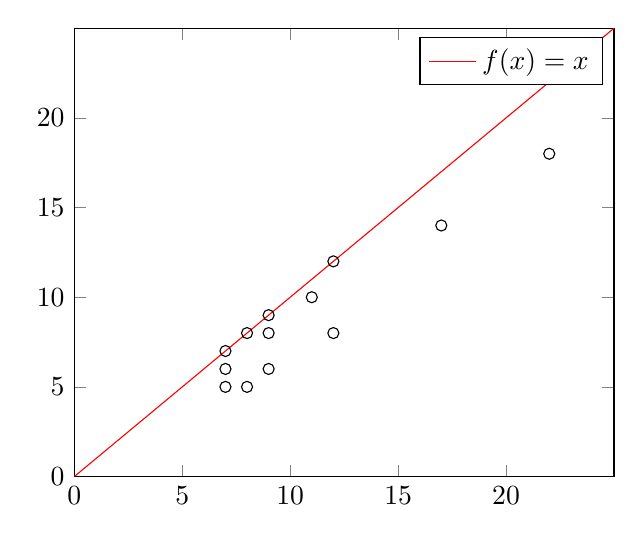
\begin{tikzpicture}
\begin{axis}[%
scatter/classes={%
a={mark=o,draw=black}},
    xmin=0, xmax=25,
    ymin=0, ymax=25,
    xtick={0, 5, 10, 15, 20},
    ytick={0, 5, 10,  15, 20},
]
\addplot [
    domain=0:25,
    color=red,
]
{x};
\addlegendentry{$f(x)=x$}
\addplot[scatter,only marks,%
    scatter src=explicit symbolic]%
table[meta=label] {
x y label
9 9 a
11 10 a
7 7 a
17 14 a
9 8 a
12 8 a
7 6 a
8 8 a
9 6 a
22 18 a
12 12 a
7 5 a
8 5 a
};

\end{axis}
\end{tikzpicture}
\caption{Each dot represents a page, with number of correct predictions on y-axis and number of connected pages on x-axis}
\end{figure}

On average 92.65\% of linked pages are correct predictions. 
Walking trough our data, we encounter three types of errors: pages that are semantically similar but are not close in a vector space, pages that are not semantically similar but are close in a vector space and technical misses. If two pages are talking about the same subject, but one of them has very little text( for example page that is mostly in pictures), their cosine score is going to be low. That type of behavior is expected from the encoder and those mistakes are acceptable. We will address them as technical misses.
On the following figure TM stands for Technical Misses, SSD for Semantically similar and distant in a vector space, NSC for not semantically similar and close in a vector space. 

\section{Future Work}

Our data set is composed of Wikipedia pages and the pages they linked to, their first neighbours. The idea is to calculate cosine similarity between every two pages. It is expected that for each page the 10 highest scores would have pages that are its first neighbours. That is however not the case and the results are inconclusive. The number of first neighbours among top 10 is not consistent and would variate from 0 to 10. \newline
Our idea is that if the data set was expanded with second and third level neighbours, these results could change. We expect in that case to find that the percentage of neighbours in top 10 dramatically increases.\newline
Another idea is try to eliminate technical misses. We know that cosine similarity depends on the quantity of text on the page. Even if the pages talk about same subject, if they have big difference in quantity of text they will be far away from each other in a vector space. We assume that we can find the coefficient that will multiply the vectors and will eliminate that difference. 

\section{Conclusion}

In this paper we tried to provide the results to prove our main idea about web's structure. We assumed the pages that were connected in webgraph would be close in a vector space. Our data showed for each page the number of correct predictions against the number of all linked pages. We showed that this correlation was linear. On average 92.65\% of linked pages were correctly predicted. Then we provided the distribution of errors showing that the most of the errors were acceptable technical misses, for which we provided the explanation. 

\begin{thebibliography}{9}
\bibitem{word2vec}
	T. Mikolov, K. Chen, G. Corrado, and J. Dean,
		\textit{Efficient estimation of word representations in vector space},
		in 1st International Conference on Learning Representations,
		ICLR 2013, 
		Scottsdale, Arizona, USA, May 2-4, 2013, Workshop Track Proceedings,
		2013.
\end{thebibliography}
\end{document}
